\normalfont\normalsize
\chapter{Testing}

The tests that we have conducted highlights the strengths of the platform but also reveals some of its weaknesses.
The most important characteristics of this experiment the maximum hight that the drone  can achieve with extra gear, the maximum range of the wireless network and the maximum range of the dongle .

Tests show the maximum range at which a drone can still communicate with base or with a SparrowV3.2,


\section{Scenario}

The testing method were conducted using a dongle with the standard antenna, a sparrowV3.2, a 3 dBi and a 8 dBi external antenna. The nodes were placed on the ground with the antenna directed upwards.

Because both the drone and nodes use 2.4 GHz network, the drone was configured to use channel 11 and the nodes to use channel 1 to prevent signal interference.

\begin{figure}[ht]
\begin{center}
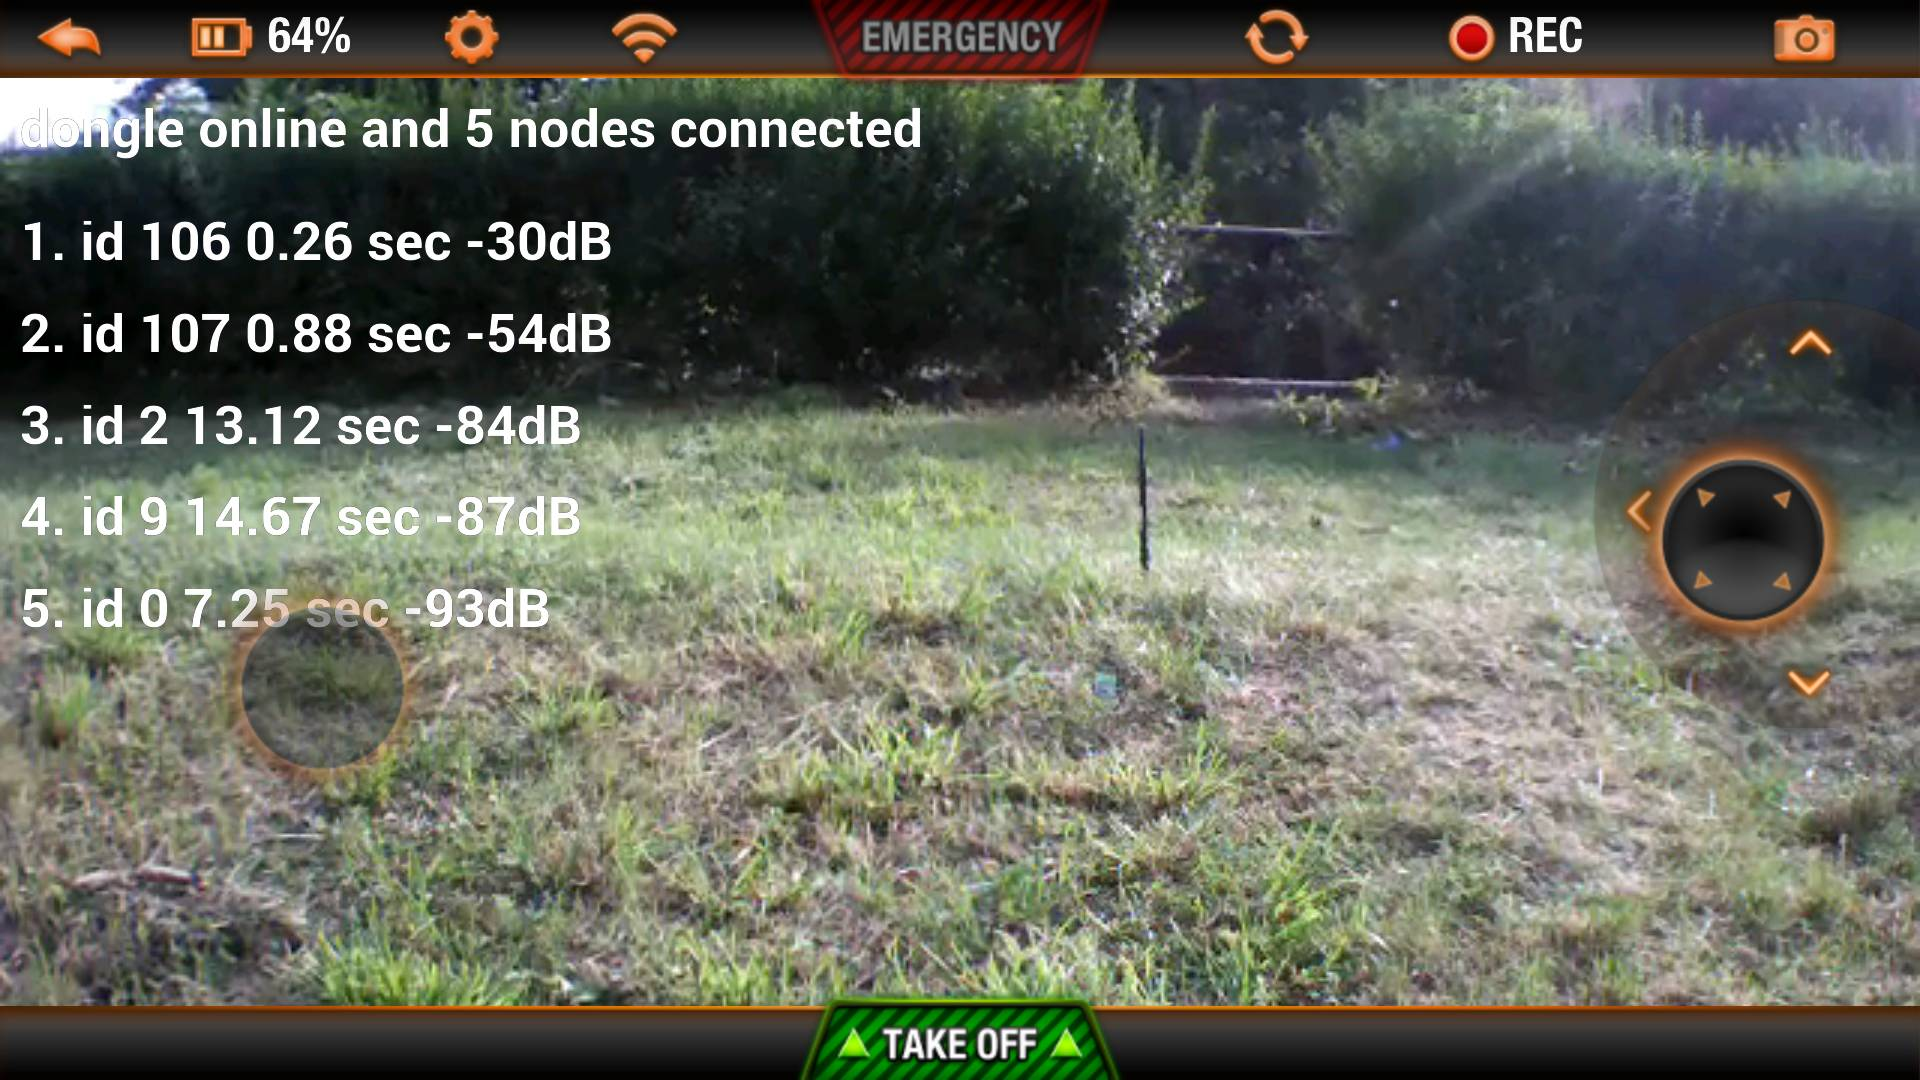
\includegraphics[width=0.45\textwidth]{img/parrot_test.png}
\end{center}
\caption{\small \itshape{Parrot discovering new nodes before takeoff}}
\end{figure}

Signal testing was performed by walking with the done in one hand and the phone in the other until the drone could not receive packets from the nodes. This test was not done by flying the drone because the exact point at which the signal is lost can not be controlled with the desired precision.



\section{Results}


\subsection{Signal range}

\begin{figure}[ht]
\begin{center}
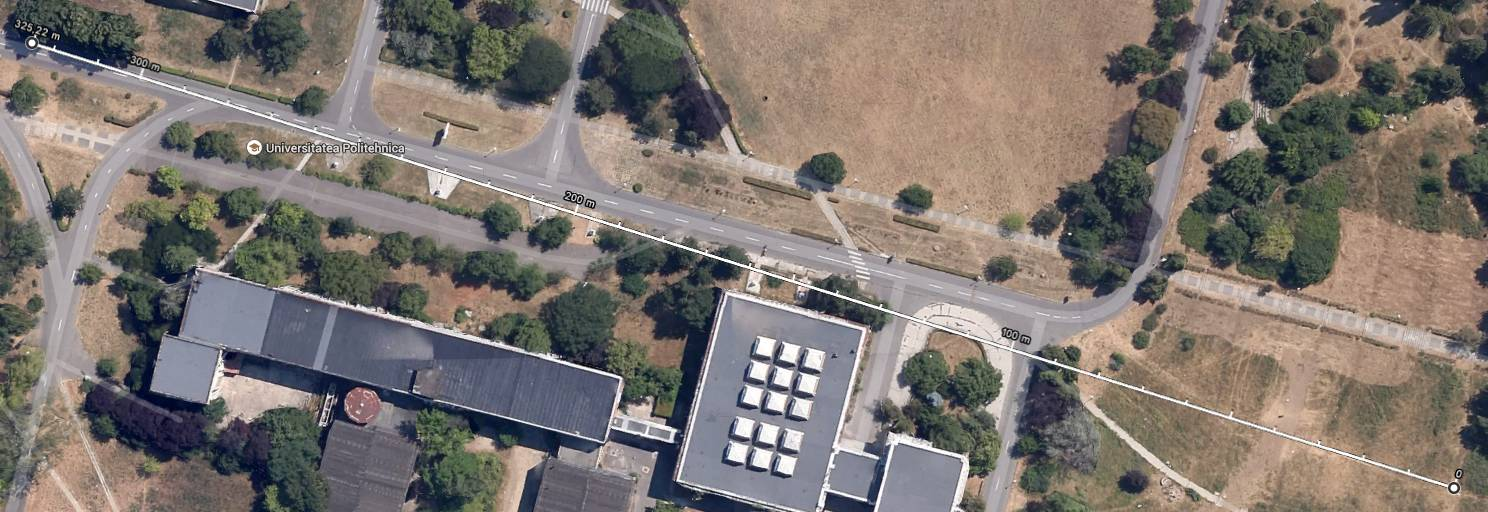
\includegraphics[width=0.9\textwidth]{img/distance.png}
\end{center}
\caption{\small \itshape{Measured signal distance}}
\end{figure}


The top mounted antenna worked, but for a better signal, the antenna should always be positioned on the bottom of the drone because in this way, the antenna will have a clear path to send and receive signal and not have the signal blocked by the entire drone and its avionics. The problem with this drone is that on the bottom of it, there are sensors that help her determine the ground speed, ground distance and the antenna could obstruct some of the sensors.

The range test results proved that the drone could receive signal from the nodes at maximum distance of 325 meters and a clear line of sight. If the node is obstructed by an object the maximum distance will decrease. For example, a node that is is placed behind an air conditioning unit and a 2 dBi antenna will have a range of just 70 meters.


\subsection{Drone stability}

Even though the antenna was mounted on top of the parrot, because it is a high gain antenna the signal received is very strong. 

The antenna extended the signal range but also added weight. The dongle is mounted on the side of the drone due to the position of the USB. Because the dongle is not centered on the drone, a counterweight had to be glued on the opposite side on the outer shell to maintain the balance of the drone. 

The drone was relatively stable during the test, but a better stability and flight control could be obtained if the dongle will be shrunk and a lighter antenna is mounted.


\begin{figure}[ht]
\begin{center}
\includegraphics[width=0.45\textwidth]{img/parrot_antenna.jpg}
\end{center}
\caption{\small \itshape{Top mounted antenna for better signal}}
\end{figure}

\begin{figure}[ht]
\begin{center}
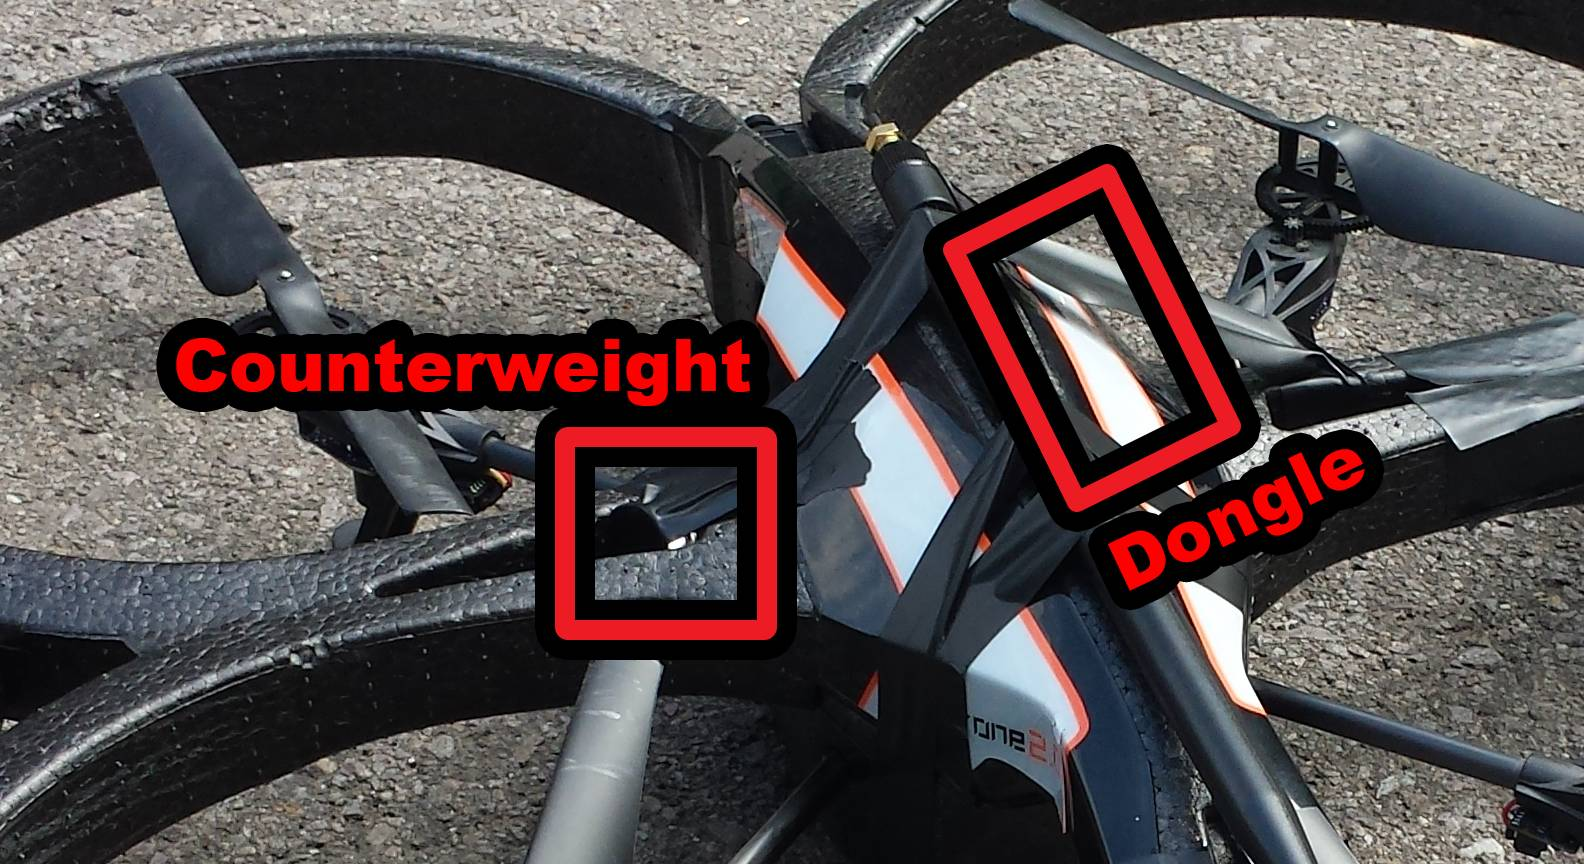
\includegraphics[width=0.45\textwidth]{img/counterweight.png}
\end{center}
\caption{\small \itshape{The counter weight need to balance the drone}}
\end{figure}

\subsection{Maximum height and maneuverability}

The total added weight is 75 grams. Even though it does not sound that much, it does have a substantial effect on the drone. The maximum height it can reach is 171784 versus the 3235 it can reach without the added weight. The maneuverability is also affected, the drone response not being as sharp as before, but it is still good.

\subsection{Problems}

The kernel module needed for the the dongle does not recognize the dongle if it is plugged in the drone when it is powered up. The fix is to power up the drone and then plug in the dongle, but this is more difficult then it might appear because every time this action is performed the hull must be repositioned.






\clearpage
 
